\documentclass{beamer}

\usetheme{metropolis}
\definecolor{mediumred}{RGB}{180, 10, 5}
\setbeamercolor{frametitle}{bg=mediumred, fg=white}

\usepackage{../../latex/tkz-graph}
\usepackage{tikz}
\usetikzlibrary{arrows,matrix,decorations.pathreplacing,positioning,chains,fit,shapes,calc} %
\usetikzlibrary{calc,patterns,decorations.pathmorphing,decorations.markings}

\usepackage{siunitx}

\usepackage{custom}
\usepackage{../../latex/jsr}

\newcommand{\expe}[2]{\la #1, #2 \ra}

\newcommand\Wider[2][3em]{%
\makebox[\linewidth][c]{%
  \begin{minipage}{\dimexpr\textwidth+#1\relax}
  \raggedright#2
  \end{minipage}%
  }%
}

\title{Computing semialgebraic invariant sets for dynamical systems}
\date{}
\author{Beno\^it Legat${}^*$, \emph{In collaboration with}: Rapha\"el M. Jungers${}^*$, Pablo A. Parrilo${}^\dagger$ and Paulo Tabuada${}^\ddagger$}
\institute{${}^*$ UCLouvain, ${}^\dagger$ MIT, ${}^\ddagger$ UCLA}

\makeatletter
\let\@@magyar@captionfix\relax
\makeatother

\begin{document}
\maketitle

  \begin{frame}
    \frametitle{Set program}
    \begin{block}{Set inclusion}
      Consider two sets $S \subseteq \R^n, T \subseteq \R^m$, matrices
      $A \in \R^{r \times n}, B \in \R^{r \times m}$,
      and vector $c \in \R^r$:
      \[ A S + c \subseteq B T. \]
    \end{block}
    \begin{block}{Set program}
    Given fixed sets $T_i$, find sets $S_i$:
    \begin{align*}
      \max_{S_i} \quad & f(\vol(S_1), \ldots, \vol(S_n))\\
      A_j S_{a_j} + c_j & \subseteq B_j S_{b_j}\\
      S_i & \subseteq T_i
    \end{align*}
    \end{block}

		\alert{Homogeneous} if $T_i$ are symmetric around the origin and $c_j = 0$.
  \end{frame}

\begin{frame}
  \frametitle{Homogenization}
	Non-homogeneous polynomial : $x^4y^2 + x^2y^4 + 1 - 3x^2y^2$.
	Homogenization : $x^4y^2 + x^2y^4 + z^6 - 3x^2y^2z^2$.

  If $T_i$ have different centers:
	Homogenization with new variable $z = 1$.
  \begin{center}
    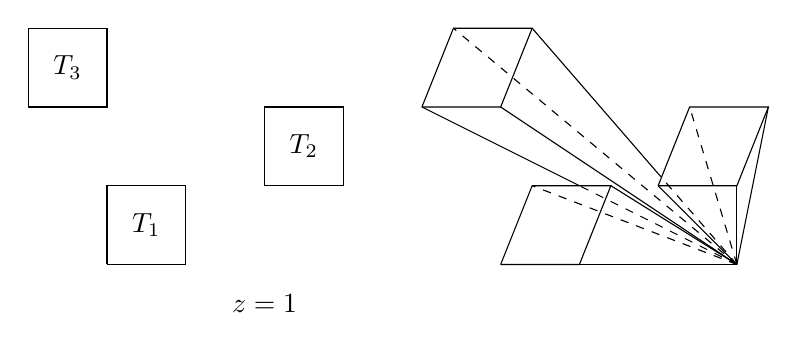
\begin{tikzpicture}
      \draw (0, 0) -- (0, 1) -- (1, 1) -- (1, 0) -- (0, 0);
      \node at (0.5, 0.5) {$T_1$};
      \draw (2, 1) -- (2, 2) -- (3, 2) -- (3, 1) -- (2, 1);
      \node at (2.5, 1.5) {$T_2$};
      \draw (-1, 2) -- (-1, 3) -- (0, 3) -- (0, 2) -- (-1, 2);
      \node at (-0.5, 2.5) {$T_3$};

      \node at (2, -0.5) {$z = 1$};
      \draw (5, 0) -- (5.4, 1) -- (6.4, 1) -- (6, 0) -- (5, 0);
      \draw[dashed] (8, 0) -- (5.4, 1);
      \draw (8, 0) -- (6.4, 1);
      \draw (8, 0) -- (6, 0);
      \draw (8, 0) -- (5, 0);
      \draw (7, 1) -- (7.4, 2) -- (8.4, 2) -- (8, 1) -- (7, 1);
      \draw (8, 0) -- (8.4, 2);
      \draw (8, 0) -- (8, 1);
      \draw (8, 0) -- (7, 1);
      \draw[dashed] (8, 0) -- (7.4, 2);
      \draw (4, 2) -- (4.4, 3) -- (5.4, 3) -- (5, 2) -- (4, 2);
      \draw[dashed] (8, 0) -- (6, 1);
      \draw (6, 1) -- (4, 2);
      \draw (8, 0) -- (5, 2);
      \draw[dashed] (8, 0) -- (7, 1.1538);
      \draw (7, 1.1538) -- (5.4, 3);
      \draw[dashed] (8, 0) -- (4.4, 3);
    \end{tikzpicture}
  \end{center}
  We now look for \alert{cones} $K$ instead of \alert{set} $S$.

  We replace \alert{polar} $S^\circ$ with \alert{dual} $K^*$.
\end{frame}

  \begin{frame}
    \frametitle{Set computation}
		Pre-image: $A^{-1} S = \{\, x \mid Ax \in S \,\}$, $A$ can be non-singular
    or rectangular.

		\begin{block}{Ellipsoid}
			\vspace{-1em}
			\begin{align*}
			  S_i & = \{\, x \mid x^\Tr Q_i x \le 1 \,\}\\
			  A^{-1} S_i & = \{\, x \mid x^\Tr A^\Tr Q_i A x \le 1 \,\}\\
			  S_i & \subseteq S_j \Leftrightarrow Q_i \succeq Q_j.
			\end{align*}
		\end{block}
			\vspace{-1em}
		\begin{block}{Polynomial sublevel set}
			\vspace{-1em}
			\begin{align*}
			  S_i & = \{\, x \mid p_i(x) \le 1 \,\}\\
			  A^{-1} S_i & = \{\, x \mid p_i(Ax) \le 1 \,\}\\
			  S_i & \subseteq S_j \Leftrightarrow p_i(x) \ge p_j(x).
			\end{align*}
		\end{block}
  \end{frame}

  \begin{frame}
    \frametitle{Set inclusions}
		\begin{block}{Simple inclusion}
      \[ A S \subseteq T \]
			we rewrite into
      \[ S \subseteq A^{-1} T \]
		\end{block}
 		\begin{block}{Polar trick}
      Inclusion with two linear maps:
      \[ A S \subseteq B T \quad \not\Leftrightarrow \quad B^{-1} S \subseteq A^{-1} T \]
			If $S$ and $T$ are convex, it is equivalent to
			\begin{align*}
        (A S)^\circ & \supseteq (B T)^\circ\\
        A^{-\Tr} S^\circ & \supseteq B^{-\Tr} T^\circ\\
			\end{align*}
		\end{block}
 \end{frame}

\begin{frame}{Controlled invariant set}
  \begin{block}{Linear discrete control system}
    \[ x_{k+1} = A x_k + B u_k, \quad x_k \in X, u_k \in U \]
  \end{block}
  \begin{block}{Controlled invariant set}
    Set $S \subseteq X$ \emph{controlled invariant} iff
    \[ \forall x \in S, \exists u \in U \text{ such that } Ax + Bu \in S \]
  \end{block}
  \begin{block}{Safe control}
    \begin{itemize}
      \item Compute controlled invariant set $S \subseteq X$.
      \item Replace $X$ by $S$.
    \end{itemize}
  \end{block}
\end{frame}

\begin{frame}{Unconstrained input without loss of generality}
  \begin{block}{\alert{Constrained} input}
    \[ x_{k+1} = A x_k + B u_k, \quad x_k \in X, \alert{u_k \in U} \]
  \end{block}
  \textbf{\alert{Lift} to \alert{un}constrained input}: $x' = (x, u)$
  \begin{align*}
    x_{k+1} & =
    \begin{pmatrix}
      A & B
    \end{pmatrix}
    x'_k\\
    u_{k+1} & =
    u'_k
  \end{align*}
  where $x'_k \in X' = X \times U$.
\end{frame}

\begin{frame}{Unconstrained control to algebraic system}
  \begin{block}{Linear Discrete \alert{Control} System (DT\alert{C}S)}
    \[ x_{k+1} = A x_k + B u_k, \quad x_k \in X \]
  \end{block}
  \begin{block}{Linear Discrete \alert{Algebraic} System (DT\alert{A}S)}
    \[ Ex_{k+1} = A x_k, \quad x_k \in X \]
    Invariant Set $S \subseteq X$ if
    \[ \forall x \in S, \alert{\exists} y \in S : Ey = Ax \]
  \end{block}
  \begin{block}{Reduction}
    The set $S$ is controlled invariant for the DT\alert{C}S iff
    it is invariant for the DT\alert{A}S
    \[ \Pi x_{k+1} = \Pi A x_k, \quad x_k \in X \]
    where $\Pi$ is a projection on $\Image(B)^\perp$.
  \end{block}
\end{frame}


\begin{frame}
  \frametitle{Computing controlled invariant sets}
  \vspace{-2em}
  \begin{align*}
    \max_S \quad & \vol(S)\\
    \Pi A S & \subseteq \Pi S\\
    S & \subseteq T
  \end{align*}
  Polar trick:
  \begin{align*}
    \min_{\polar{S}} \quad & \vol(\polar{S})\\
    (\Pi A)^{-\Tr} \polar{S} & \supseteq \Pi^{-\Tr} \polar{S}\\
    \polar{S} & \supseteq \polar{T}
  \end{align*}
  Suppose $T = \{\,x : |\langle h_i, x \rangle| \leq 1\,\}$, using ellipsoids
  \begin{align*}
    \min_{Q \succ 0} \quad & -\log \det(Q)\\
    \Pi A Q A^\Tr \Pi^\Tr & \preceq \Pi Q \Pi^\Tr\\
    h_i^\Tr Q h_i & \le 1 \qquad \forall i
  \end{align*}
\end{frame}

\begin{frame}{Safety in control requires \alert{long} horizon}
  Speed limit changes from \SI{35}{\meter\per\second} to \SI{15.6}{\meter\per\second} after \SI{30}{\second}.
  \begin{center}
    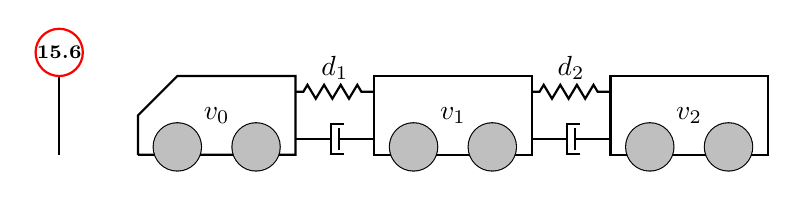
\begin{tikzpicture}
      \tikzstyle{spring}=[thick,decorate,decoration={zigzag,pre length=0.1cm,post length=0.1cm,segment length=6}]
\tikzstyle{damper}=[thick,decoration={markings,
  mark connection node=dmp,
  mark=at position 0.5 with
  {
    \node (dmp) [thick,inner sep=0pt,transform shape,rotate=-90,minimum width=10pt,minimum height=2pt,draw=none] {};
    \draw [thick] ($(dmp.north east)+(2pt,0)$) -- (dmp.south east) -- (dmp.south west) -- ($(dmp.north west)+(2pt,0)$);
    \draw [thick] ($(dmp.north)+(0,-4pt)$) -- ($(dmp.north)+(0,4pt)$);
  }
}, decorate]
\draw[thick] (0, 0) -- (2, 0) -- (2, 1) -- (0.5, 1) -- (0, 0.5) -- (0, 0);
\draw [spring] (2, 0.8) -- (3, 0.8);
\draw [damper] (2, 0.2) -- (3, 0.2);
\draw[thick] (3, 0) rectangle (5, 1);
\draw [spring] (5, 0.8) -- (6, 0.8);
\draw [damper] (5, 0.2) -- (6, 0.2);
\draw[thick] (6, 0) rectangle (8, 1);
\draw[thick] (0.5, 0.1) circle (0.3);
\fill[color=lightgray] (0.5, 0.1) circle (0.3);
\draw[thick] (1.5, 0.1) circle (0.3);
\fill[color=lightgray] (1.5, 0.1) circle (0.3);
\draw[thick] (3.5, 0.1) circle (0.3);
\fill[color=lightgray] (3.5, 0.1) circle (0.3);
\draw[thick] (4.5, 0.1) circle (0.3);
\fill[color=lightgray] (4.5, 0.1) circle (0.3);
\draw[thick] (6.5, 0.1) circle (0.3);
\fill[color=lightgray] (6.5, 0.1) circle (0.3);
\draw[thick] (7.5, 0.1) circle (0.3);
\fill[color=lightgray] (7.5, 0.1) circle (0.3);
\node at (1, 0.5) {$v_0$};
\node at (4, 0.5) {$v_1$};
\node at (7, 0.5) {$v_2$};
\node at (2.5, 1.1) {$d_1$};
\node at (5.5, 1.1) {$d_2$};

      \draw[thick] (-1, 0) to (-1, 1);
      \draw[thick,color=red] (-1, 1.3) circle (0.3);
      \node at (-1, 1.3) {\scriptsize \bf 15.6};
    \end{tikzpicture}
  \end{center}
  One trailer, step-size of \SI{0.4}{\second}, horizon of \SI{9.2}{\second}/23 step-sizes:
  \begin{center}
    \includegraphics[width=0.5\textwidth]{CruiseControlUnsafeSpeed.pdf}~%
    \includegraphics[width=0.5\textwidth]{CruiseControlUnsafeAcceleration.pdf}
  \end{center}
\end{frame}

\begin{frame}{Controlled invariant set}
  \begin{columns}
    \begin{column}{0.55\textwidth}
      \begin{center}
        \includegraphics[width=\textwidth]{CruiseControlSets.pdf}
        \includegraphics[width=\textwidth]{CruiseControlBenchmark.png}
      \end{center}
    \end{column}
    \begin{column}{0.55\textwidth}
      \begin{center}
        \includegraphics[width=\textwidth]{CruiseControlSpeed.pdf}
        \includegraphics[width=\textwidth]{CruiseControlAcceleration.pdf}
      \end{center}
    \end{column}
  \end{columns}
\end{frame}

\begin{frame}
  \frametitle{Water Reservoir}
  \begin{itemize}
    \item $h_{\textnormal{min}} \le h \le h_{\textnormal{max}}$ : water height [\si{\meter}]
    \item $v_{\textnormal{min}} \le v \le v_{\textnormal{max}}$ : height increase rate [\si{\meter\per\second}]
    \item $u_{\textnormal{min}} \le u \le u_{\textnormal{max}}$ : $v$ increase rate [\si{\meter\per\second\squared}]
  \end{itemize}
  \begin{columns}
    \begin{column}{0.45\textwidth}
      \begin{itemize}
        \item $h > h_{\textnormal{max}}$: Water \alert{spills}, ecological damage
        \item $h < h_{\textnormal{min}}$: Risk of electricity \alert{shortage}
      \end{itemize}
    \end{column}
    \begin{column}{0.45\textwidth}
      \begin{center}
        \includegraphics[width=\textwidth]{reservoir.jpg}
      \end{center}
    \end{column}
  \end{columns}
\end{frame}

\begin{frame}
  \frametitle{Controlled invariant set}
  \begin{center}
    \includegraphics[trim=.2cm .2cm .2cm .2cm, clip, width=\textwidth]{ReservoirEllipsoidal.pdf}
  \end{center}
\end{frame}

  \begin{frame}
      \frametitle{Joint Spectral Radius and Switched Systems}
      \begin{block}{Switched Systems}
      \vspace{-.5em}
        \[ x_{k+1} = A_{\sigma_k} x_k, \qquad \sigma_k \in \{1, \ldots, m\}. \]
      \end{block}
      \vspace{-1em}
          \hspace{2em}
          Switched System \alert{stable}
          \hspace{1em}
          $\Longleftrightarrow$%
          \hspace{1em}
          $\lim_{k \to \infty} x_k = 0$ $\forall x_0$.
      \uncover<2->{
      \begin{block}{Joint Spectral Radius (JSR) $\A = \{A_1, \ldots, A_m\}$}
      \vspace{-.5em}
        \[ \rho(\A) := \limsup_{k\to\infty} \max_{\sigma \in \{1,\ldots,m\}} \norm{A_{\sigma_k} \cdots A_{\sigma_2}A_{\sigma_1}}^{1/k}. \]
      \end{block}
      \vspace{-1em}
          \hspace{2em}
          Switched System \alert{stable}
          \hspace{1em}
          $\Longleftrightarrow$%
          \hspace{1em}
          $\rho(\A) < 1$
      }

      \uncover<3->{
      \begin{itemize}
        \item If $m = 1$, ``standard'' spectral radius $\rho(A_1) = \max_i |\lambda_i|$.
        \uncover<4->{
        \item If $m \geq 2$, much more complicated...
          \begin{itemize}
            \uncover<4->{\item Determining if $\rho(\A) < 1$ is \alert{NP-hard} (Tsitsiklis \& Blondel 1997).}
            \uncover<4->{\item Determining if $\rho(\A) \leq 1$ is \alert{undecidable} (Blondel \& Tsitsiklis 2000).}
          \end{itemize}
        }
      \end{itemize}
      }
  \end{frame}

  \begin{frame}
    \frametitle{Joint Spectral Radius and Invariant Sets}
    \begin{block}{Invariant Set}
      \vspace{-.5em}
      \[ A_\sigma S \in S, \sigma \in \{1, \ldots, m\} \]
    \end{block}
      \vspace{-1.5em}
    \begin{example}
      \vspace{-1em}
      $m = 1$, $A_1 = \text{Rotation}(\ang{90}) \times \begin{pmatrix}0.5 & 0\\0 & 2\end{pmatrix}$
      \vspace{-1em}
      \begin{center}
        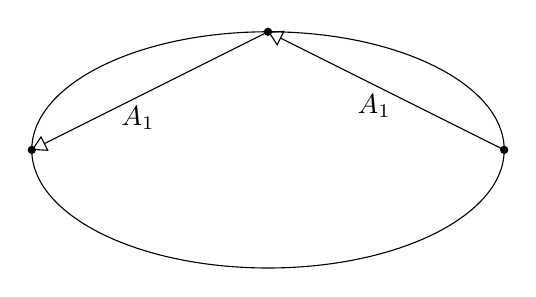
\begin{tikzpicture}[scale=1.5]
          \draw (0, 0) ellipse (2 and 1);
          \draw[fill] (2, 0) circle (0.03);
          \draw[fill] (0, 1) circle (0.03);
          \draw[-open triangle 60] (2, 0) to node[below,pos=0.55] {$A_1$} (0, 1);
          \draw[-open triangle 60] (0, 1) to node[below,pos=0.55] {$A_1$} (-2, 0);
          \draw[fill] (-2, 0) circle (0.03);
        \end{tikzpicture}
      \end{center}
    \end{example}

    \uncover<2->{
      \hspace{1em}
      $\exists$ invariant set for $A_1/\gamma, \ldots, A_m/\gamma$
      \hspace{1em}
      $\Longrightarrow$%
      \hspace{1em}
      $\rho(\A) \leq \gamma$
    }

    \uncover<3->{
      \hspace{1em}
      $\exists$ invariant set for $A_1/\gamma, \ldots, A_m/\gamma$
      \hspace{1em}
      $\Longleftarrow$%
      \hspace{1em}
      $\rho(\A) < \gamma$
    }
  \end{frame}

  \begin{frame}
    \frametitle{SOS-$2d$ invariant sets}
    Can compute invariant sets using Sum of Squares Programming (SOS) :
    $S = \{\, x : p(x) \leq 1\,\}$ where $p(x)$ homogeneous %
    SOS degree $2d$.

    \uncover<2->{
      \begin{block}{Guarantee}
        \[
          \ujsrsos =
          \begin{aligned}
            \inf \,\,& \gamma\\
            \text{s.t.}\,\, & \exists \text{ SOS-$2d$ invariant set for } A_1/\gamma, \ldots, A_m/\gamma
          \end{aligned}
        \]
        \[ \eta^{-\frac{1}{2d}} \ujsrsos \leq \jsr \leq \ujsrsos \]
        where $\eta = \min\Big\{m, {n+d-1 \choose d}\Big\}$ and $A_\sigma \in \R^{n \times n}$.

        As $d \to \infty$, $\eta^{-\frac{1}{2d}} \to 0$.
      \end{block}
    }
    \vfill
    {\scriptsize
    P.A. Parrilo and A. Jadbabaie,
    Approximation of the joint spectral radius using sum of squares,
    \emph{Linear Algebra and its Applications},
    Vol. 428, No. 10, pp.~2385--2402, 2008.
    }
  \end{frame}

  \begin{frame}{Measures}
    Measures $\mu$ defined on the sphere
    \[
      \Sn = \{\, x : \norm{x}_2 = 1\,\}
    \]
    For $B \in \Sn$, $\mu(B)$ is \alert{measure} of $B$.

    \alert{atomic} $\Leftrightarrow$ sum of \alert{Diracs}

    \alert{amplitude} in drawing represents
    \begin{itemize}
      \item \alert{mass} of atom for \emph{atomic} measure,
      \item \alert{density} otherwise.
    \end{itemize}
    \vspace{-1.2em}
    \begin{center}
      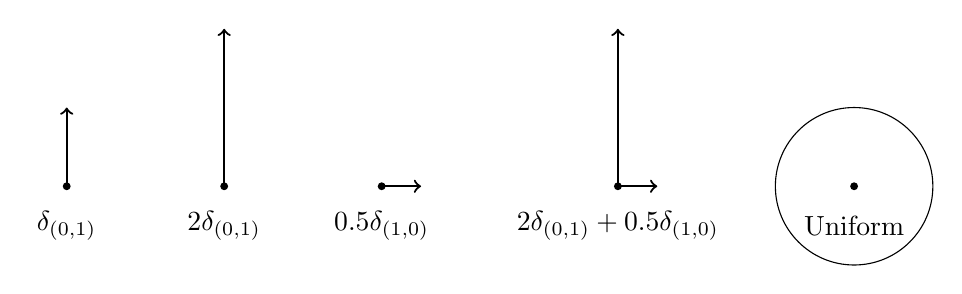
\begin{tikzpicture}
        \begin{scope}[shift={(-4,0)}]
          \draw[thick,->] (0,0) to (0,1);
          \fill (0,0) circle(.05);
          \node at (0,-.5) {$\delta_{(0, 1)}$};
        \end{scope}
        \begin{scope}[shift={(-2,0)}]
          \draw[thick,->] (0,0) to (0,2);
          \fill (0,0) circle(.05);
          \node at (0,-.5) {$2\delta_{(0, 1)}$};
        \end{scope}
        \begin{scope}[shift={(0,0)}]
          \draw[thick,->] (0,0) to (0.5,0);
          \fill (0,0) circle(.05);
          \node at (0,-.5) {$0.5\delta_{(1, 0)}$};
        \end{scope}
        \begin{scope}[shift={(3,0)}]
          \draw[thick,->] (0,0) to (0,2);
          \draw[thick,->] (0,0) to (0.5,0);
          \fill (0,0) circle(.05);
          \node at (0,-.5) {$2\delta_{(0, 1)} + 0.5\delta_{(1, 0)}$};
        \end{scope}
        \begin{scope}[shift={(6,0)}]
          \draw (0,0) circle(1);
          \fill (0,0) circle(.05);
          \node at (0,-.5) {Uniform};
        \end{scope}
      \end{tikzpicture}
    \end{center}
  \end{frame}

  \begin{frame}{Transfer/Frobenius-Perron operator and push-forward measure}
    Usual definition:
    \[ (\pushf{A}{\mu})(B) = \mu(A^{-1}(B)) \]
    \alert{Problem}: $\Sn$ not invariant under $A_\sigma$.

    \alert{Solution}: Alternative definition:
    \[ \int_{\Sn} f(x) (\pushf{A}{\mu})(\dif x) = \int_{\Sn} f(Ax) \mu(\dif x) \qquad \forall f. \]

    \begin{example}
      $A_1 = \text{Rotation}(\ang{90}) \times \begin{pmatrix}0.5 & 0\\0 & 2\end{pmatrix}$
      \begin{center}
        \begin{tikzpicture}
          \begin{scope}[shift={(-3,0)}]
            \draw[thick,->] (0,0) to (0,1);
            \draw[thick,->] (0,0) to (1,0);
            \fill (0,0) circle(.05);
            \node at (0,-.5) {$\mu$};
          \end{scope}
          \begin{scope}[shift={(4,0)}]
            \draw[thick,->] (0,0) to (-2,0);
            \draw[thick,->] (0,0) to (0,0.5);
            \fill (0,0) circle(.05);
            \node at (0,-.5) {$\pushf{A}{\mu}$};
          \end{scope}
        \end{tikzpicture}
      \end{center}
    \end{example}
  \end{frame}

  \begin{frame}{Periodic trajectory}
    \alert{Periodic} trajectory of growth rate $\gamma$:
    \[ \gamma^k x_0 = A^k x_0 \]
    $\exists x_i$, $1 \leq i \leq k$, such that:
    \[ \gamma x_{i+1} = A x_i \]

    \begin{example}
      \vspace{-1em}
      $A = \text{Rotation}(\ang{90}) \times \begin{pmatrix}0.5 & 0\\0 & 2\end{pmatrix}$,
      $x_0 = (1, 0)$, $k = 4$
      \vspace{-1em}
      \begin{center}
        \begin{tikzpicture}[scale=1.5]
          \draw[thick,->] (0,0) to (2,0);
          \node[above] at (2,0) {$x_0 = x_4$};
          \draw[thick,->] (0,0) to (0,1);
          \node[right] at (0,1) {$x_1$};
          \draw[thick,->] (0,0) to (-2,0);
          \node[below] at (-2,0) {$x_2$};
          \draw[thick,->] (0,0) to (0,-1);
          \node[left] at (0,-1) {$x_3$};
        \end{tikzpicture}
      \end{center}
    \end{example}
  \end{frame}

  \begin{frame}{Periodic trajectory as atomic measure I}
    Equivalent to:
    \[ \gamma \delta_{x_{k+1}} = \pushf{A}{\delta_{x_k}} \]

    \begin{example}
      \vspace{-1em}
      $A = \text{Rotation}(\ang{90}) \times \begin{pmatrix}0.5 & 0\\0 & 2\end{pmatrix}$,
      $x_0 = (1, 0)$, $k = 4$
      \vspace{-1em}
      \begin{center}
        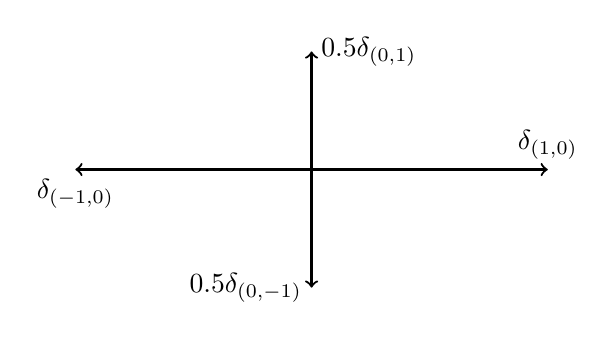
\begin{tikzpicture}[scale=1.5]
          \draw[thick,->] (0,0) to (2,0);
          \node[above] at (2,0) {$\delta_{(1,0)}$};
          \draw[thick,->] (0,0) to (0,1);
          \node[right] at (0,1) {$0.5\delta_{(0,1)}$};
          \draw[thick,->] (0,0) to (-2,0);
          \node[below] at (-2,0) {$\delta_{(-1,0)}$};
          \draw[thick,->] (0,0) to (0,-1);
          \node[left] at (0,-1) {$0.5\delta_{(0,-1)}$};
        \end{tikzpicture}
      \end{center}
    \end{example}
  \end{frame}

  \begin{frame}{Periodic trajectory as atomic measure II}
    \alert{Convex}ification: Find $\mu_{k}$ such that for all $k = 1, \ldots$
    \[ \gamma \mu_{k+1} = \pushf{A}{\mu_k}. \]
    Project the time:
    \[ \gamma \mu = \pushf{A}{\mu}. \]

    \begin{example}
      \vspace{-1em}
      $A = \text{Rotation}(\ang{90}) \times \begin{pmatrix}0.5 & 0\\0 & 2\end{pmatrix}$,
      $x_0 = (1, 0)$, $k = 4$
      \vspace{-1em}
      \begin{center}
        \begin{tikzpicture}[scale=1.5]
          \draw[thick,->] (0,0) to (2,0);
          \draw[thick,->] (0,0) to (0,1);
          \draw[thick,->] (0,0) to (-2,0);
          \draw[thick,->] (0,0) to (0,-1);
          \node at (0,-1.3) {$\mu = \pushf{A}{\mu}$};
        \end{tikzpicture}
      \end{center}
    \end{example}
  \end{frame}

  \begin{frame}{Periodic trajectory as atomic measure III}
    \[ \gamma (\mu_1 + \mu_2) = \pushf{A_1}{\mu_1} + \pushf{A_2}{\mu_2}. \]

    \alert{periodic} trajectory of growth rate $\gamma$ $\leftrightarrow$ \alert{atomic} measures.

    \begin{example}
  \vspace{-1em}
  \begin{align*}
      A_1 & =
      \begin{bmatrix}
          0 & 2\\
          0 & 0
      \end{bmatrix}&
      A_2 & =
      \begin{bmatrix}
          0 & 0\\
          2 & 0
      \end{bmatrix}
  \end{align*}
  \vspace{-2em}
  \begin{center}
    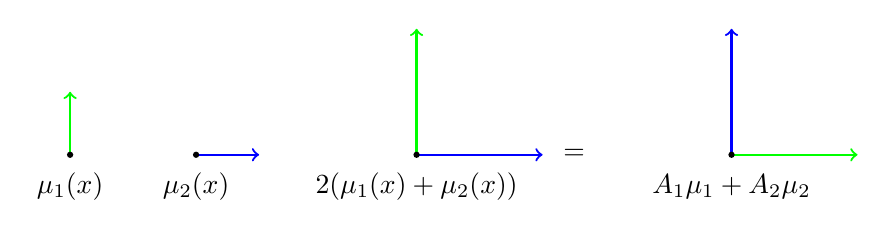
\begin{tikzpicture}[scale=0.8]
        \begin{scope}[shift={(-8,0)}]
            \draw[thick,->,green] (0,0) to (0,1);
            \fill (0,0) circle(.05);
            \node at (0,-.5) {$\mu_1(x)$};
        \end{scope}

        \begin{scope}[shift={(-6,0)}]
            \draw[thick,->,blue] (0,0) to (1,0);
            \fill (0,0) circle(.05);
            \node at (0,-.5) {$\mu_2(x)$};
        \end{scope}

        \begin{scope}[shift={(-2.5,0)}]
            \draw[thick,->,green] (0,0) to (0,2);
            \draw[thick,->,blue] (0,0) to (2,0);
            \fill (0,0) circle(.05);
            \node at (0,-.5) {$2(\mu_1(x) + \mu_2(x))$};
        \end{scope}

        \begin{scope}[shift={(0,0)}]
            \node at (0,0) {$=$};
        \end{scope}

        \begin{scope}[shift={(2.5,0)}]
            \draw[thick,->,green] (0,0) to (2,0);
            \draw[thick,->,blue] (0,0) to (0,2);
            \fill (0,0) circle(.05);
            \node at (0,-.5) {$\pushf{A_1}{\mu_1} + \pushf{A_2}{\mu_2}$};
        \end{scope}
    \end{tikzpicture}
  \end{center}
\end{example}

  \end{frame}

  \begin{frame}{Joint Spectral Radius and Invariant Measures}
    \begin{block}{Theorem}
      Let $\mu_{\sigma}$, $\sigma=1, \ldots, m$, be measures on $\mathbb{S}^{n-1}$,
      that satisfies
      \[ \sum_{\sigma = 1}^m \pushf{A_\sigma}{\mu_\sigma} \geq \gamma \sum_{\sigma = 1}^m \mu_\sigma, \]
      and at least one of the expectations is nonzero.

      Then  $\jsr \geq \gamma$.
    \end{block}
  \end{frame}

  \begin{frame}{SOS-$2d$ invariant measures}
    \alert{Moments} $\pmu$ of degree $2d$.
    Can write constraint
    \[
        \la \pmu, p(x) \ra = \int_{\mathbb{S}^{n-1}} p(x) \dif \pmu \geq 0, \qquad \forall p(x) \text{ SOS of degree }2d.
    \]
    as Semidefinite Programming constraint. %

    \alert{Dual} to invariant sets program.

    \uncover<2->{
      \begin{itemize}
        \item Can detect when moments of \alert{atomic} measures and recover
          atoms by solving an algebraic system.
          The moments are computed numerically with errors around $10^{-6}$,
          currently doing Gr\"obner basis computation in double precision
          floating point numbers in Julia. We should try \jlpkg{HomotopyContinuation}.
        \item \alert{relaxation}: can have moments of no measure ! But... \uncover<3>{\alert{pseudo-measure}
            \[ \expe{\pmu}{p(x)} \geq 0, \quad \forall p(x) \text{ SOS}. \]
          }
      \end{itemize}
    }
  \end{frame}

  \begin{frame}{Making a liar tell the truth}
    If \alert{atomic}, take $x_0$:
    \[ \sigma_{k+1} = \argmax_\sigma \mu_\sigma(\{x_k/\norm{x_k}_2\}), \quad x_{k+1} = A_{\sigma_{k+1}} x_k \]

    \vspace{-1.5em}
    \begin{example}
  \vspace{-1em}
  \begin{align*}
      A_1 & =
      \begin{bmatrix}
          0 & 2\\
          0 & 0
      \end{bmatrix}&
      A_2 & =
      \begin{bmatrix}
          0 & 0\\
          2 & 0
      \end{bmatrix}
  \end{align*}
  \vspace{-2em}
  \begin{center}
    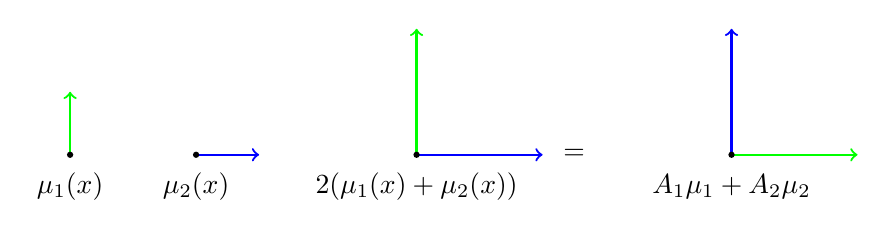
\begin{tikzpicture}[scale=0.8]
        \begin{scope}[shift={(-8,0)}]
            \draw[thick,->,green] (0,0) to (0,1);
            \fill (0,0) circle(.05);
            \node at (0,-.5) {$\mu_1(x)$};
        \end{scope}

        \begin{scope}[shift={(-6,0)}]
            \draw[thick,->,blue] (0,0) to (1,0);
            \fill (0,0) circle(.05);
            \node at (0,-.5) {$\mu_2(x)$};
        \end{scope}

        \begin{scope}[shift={(-2.5,0)}]
            \draw[thick,->,green] (0,0) to (0,2);
            \draw[thick,->,blue] (0,0) to (2,0);
            \fill (0,0) circle(.05);
            \node at (0,-.5) {$2(\mu_1(x) + \mu_2(x))$};
        \end{scope}

        \begin{scope}[shift={(0,0)}]
            \node at (0,0) {$=$};
        \end{scope}

        \begin{scope}[shift={(2.5,0)}]
            \draw[thick,->,green] (0,0) to (2,0);
            \draw[thick,->,blue] (0,0) to (0,2);
            \fill (0,0) circle(.05);
            \node at (0,-.5) {$\pushf{A_1}{\mu_1} + \pushf{A_2}{\mu_2}$};
        \end{scope}
    \end{tikzpicture}
  \end{center}
\end{example}

    \vspace{-1.5em}
    If \alert{pseudo-measure}, take $p_0(x)$ SOS:
    \[ \sigma_{k+1} = \argmax_\sigma \expe{\mu_\sigma}{p_k(x)}, \quad p_{k+1}(x) = p_k(A_{\sigma_{k+1}} x) \]
    \textbf{Note}: Switching built \alert{backward}!
  \end{frame}

  \begin{frame}{Infinite backward sequence}
    \begin{alert}{Guarantee}
      \[ m^{-\frac{1}{2d}}\ujsrsos \leq \lim_{k \to \infty} \norm{A_{\sigma_1} \cdots A_{\sigma_k}}^{\frac{1}{k}} \leq \jsr \leq \ujsrsos. \]
    \end{alert}

    If sequence \alert{periodic} $\to$ can compute growth rate

    \vfill

    {\scriptsize
    B. L., R.M. Jungers and P.A. Parrilo,
    Generating unstable trajectories for Switched Systems via Dual Sum-Of-Squares techniques,
    \emph{Proceedings of the 19th International Conference on Hybrid Systems: Computation and Control},
    ACM, pp.~51--60, 2016.
    }
  \end{frame}
  \begin{frame}{Constraint Joint Sectral Radius}
\Wider{
    For set program with several $S_i$, consider the graph where nodes are $S_i$
    and edges are constraints $A_{\sigma_j} S_{a_j} \subseteq S_{b_j}$

    Allowed switching sequences $\sigma_1, \sigma_2, \ldots$ $\leftrightarrow$ paths of graph.

    \[ \rho(\Adj)^{-\frac{1}{2d}}\jsrsos \leq \lim_{k \to \infty} \norm{A_{\sigma_1} \cdots A_{\sigma_k}}^{\frac{1}{k}} \leq \cjsr \leq \jsrsos. \]
    where $\Adj$ is adjacency matrix of the graph.
}
  \end{frame}
  \begin{frame}{Conclusion}
    \begin{itemize}
      \item Set programs can be solved using sum of squares programming
      \item This can be used to compute controlled invariant sets.
      \item With simple inclusion and homogeneity, infeasibility can be certificied using the dual.
    \end{itemize}
  \end{frame}

\end{document}
